\documentclass[conference]{IEEEtran}
\IEEEoverridecommandlockouts
% The preceding line is only needed to identify funding in the first footnote. If that is unneeded, please comment it out.
\usepackage{cite}
\usepackage{amsmath,amssymb,amsfonts}
\usepackage{algorithmic}
\usepackage{graphicx}
\usepackage{textcomp}
\usepackage{xcolor}
\usepackage{hyperref}
\def\BibTeX{{\rm B\kern-.05em{\sc i\kern-.025em b}\kern-.08em
    T\kern-.1667em\lower.7ex\hbox{E}\kern-.125emX}}
\begin{document}

\title{Streaming Audiovisual: uma análise como sistema de informação}

\author{\IEEEauthorblockN{Gustavo Henrique Ferreira Alves}
\IEEEauthorblockA{\textit{Graduando em Sistemas de Informação} \\
\textit{Universidade de São Paulo}\\
São Paulo, Brasil \\}
\and
\IEEEauthorblockN{Kevin Rodrigues Nunes}
\IEEEauthorblockA{\textit{Graduando em Sistemas de Informação} \\
\textit{Universidade de São Paulo}\\
São Paulo, Brasil \\}
}

\maketitle

\begin{abstract}

As plataformas de streaming audiovisual se tornaram Sistemas de Informação essenciais na indústria de comunicação e entretenimento, facilitando a entrega global de conteúdo com sistemas de recomendação que utilizam análise de dados e aprendizado de máquina para prever preferências dos usuários e otimizar ofertas de conteúdo. Empresas como Spotify e Netflix transformaram o consumo cultural e introduziram novos modelos de monetização, forçando tradicionais do entretenimento a adotarem o streaming. O artigo analisa essas plataformas como Sistemas de Informação, destacando a integração tecnológica e algoritmos de recomendação, além de seu impacto em estratégias de mercado e operações. Também aborda a interação entre hardware, software e recursos humanos, e discute questões éticas relacionadas à privacidade dos dados, impacto ambiental e manipulação de usuários, apontando para a necessidade de supervisão regulatória. Desse modo, conclui-se que as plataformas de streaming exemplificam princípios fundamentais dos Sistemas de Informação e influenciam significativamente o consumo cultural e a indústria do entretenimento.\end{abstract}


\begin{IEEEkeywords}
streaming, sistemas de recomendação, sistemas de informação, netflix, spotify, audiovisual
\end{IEEEkeywords}

\section{Introdução}
As plataformas de streaming audiovisuais são Sistemas de Informação que se tornaram de suma importância para o atual cenário da indústria de comunicação e entretenimento. Envolvendo técnicas e partes complexas, suas funções são de garantir a solicitação e entrega de conteúdos audiovisuais para usuários em escala global, contando, para isso, com robustos sistemas de recomendação que incorporam técnicas avançadas de análise de dados e aprendizado de máquina para prever tendências e preferências dos usuários, otimizando a oferta de conteúdo e maximizando a retenção de assinantes \cite{b1}.

Popularizadas por empresas não tradicionais como Spotify e Netflix, suas implementações não só mudaram a forma em que a sociedade consome a produção cultural audiovisual, como também impulsionou novas formas de monetização, como modelos de assinatura, publicidade segmentada e transações pay-per-view, obrigando indústrias tradicionais do ramo de entretenimento a entregar seus produtos através desse tipo de sistema, como ocorreu com a WarnerMedia e a The Walt Disney Company \cite{b2}.

Assim, ao analisar as plataformas de streaming como Sistemas de Informação, é crucial entender como cada componente – desde técnicas de entrega audiovisual até os algoritmos de recomendação – se interconecta para fornecer um serviço que não só atende às demandas contemporâneas dos consumidores, mas também redefine as estratégias operacionais e de mercado das empresas no setor de entretenimento. A capacidade dessas plataformas de integrar diferentes formas de mídia, como vídeos, músicas e jogos, contribui para a criação de um ecossistema interdependente que aumenta o engajamento e diversifica as fontes de receita \cite{b1} \cite{b2}.
\section{Categorizando como um Sistema de Informação}

Temos por definição que "Sistemas de Informação são componentes inter-relacionados que coletam (ou recuperam), processam, armazenam e distribuem informações destinadas a apoiar a tomada de decisões, a coordenação e o controle de uma organização" \cite{b3}\footnote{Ver p. 9.}. Com esse ponto de partida, podemos analisar, ação por ação, como a plataforma de streaming audiovisual, alinhada com o sistema de recomendação, se enquadra nessa categoria de sistema.

\subsection{Identificando seus componentes: Streaming}
\subsubsection{Software, Hardware e Pessoas}
\label{sec: Software, Hardware e Pessoas}
A priori, é necessário entender os componentes que integram as plataformas de streaming audiovisual. Em termos funcionais, são muitas as tecnologias que sustentam seu funcionamento. Em 2007, quando a Netflix reformulou a estrutura empresarial a fim de introduzir o streaming como alternativa aos seus negócios de venda e aluguel de DVD’s \cite{b4} foi, paralelamente, desenvolvido pela Move Networks a entrega de arquivos através do protocolo HTTP \cite{b5}, tecnologia essa que foi aprimorada e relançada por diversas empresas de tecnologia. Atualmente, derivadas dessa técnica de entrega, temos como dominante no mercado o HLS (HTTP Live Streaming) - desenvolvido pela empresa Apple - e o MPEG-DASH (Dynamic Adaptative Streaming over HTTP), protocolo aberto desenvolvido pela MPEG. A partir de qualquer um desses protocolos, que repartem os arquivos de vídeo e áudio e entregam-nos em pequenas partes em sequência, é necessário integrar o processo com a tecnologia de CDN (Content Delivery Network), que por sua vez possibilitará a entrega em grandes escalas de alcance.

\begin{figure}[htbp]
\centerline{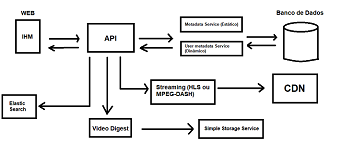
\includegraphics{fig1.png}}
\caption{Arquitetura do Streaming.}
\label{fig}
\end{figure}

Os arquivos que são repartidos pelos protocolos de entrega HTTP devem ser armazenados na íntegra e na máxima resolução possível. Para isso são desenvolvidos bancos de dados que, além de guardar os arquivos, os associam com serviços de metadados onde contenham informações ao seu respeito, como: título, duração, gênero e autores. Esses dados estáticos são extremamente necessários para a identificação nas IHM's do sistema. Além destes, os bancos de dados também devem ser projetados para suportar entradas de dados dinâmicas relacionadas aos usuários do sistema.

Para sustentar esses componentes baseados em software, a plataforma de streaming necessita de uma grande capacidade de hardware e um grande número de pessoas, principalmente quando são plataformas de alta perfomance, como a Netflix, o Spotify ou HBO Max. No que tange o componente hardware, é importante salientar que muitas organizações que se beneficiam do streaming terceirizam essa parte do SI, utilizando como alternativa serviços em nuvem como AWS, Azure ou Oracle. Em detalhes, são necessários: 

\begin{itemize}
\item Servidores de Armazenamento e Processamento: Estes dispositivos físicos hospedam e entregam o conteúdo aos usuários. Para este fim, é necessário que sejam velozes em processamento e escaláveis, para suportar grandes quantidades de tráfego de dados simultâneos.
\item Equipamentos de Redes: Referem-se a roteadores, switches, firewalls e outros equipamentos usados para gerenciar o tráfego de dados entre os diferentes componentes do sistema de informação, garantindo uma comunicação que, além de eficiente, seja segura.
\end{itemize}

Quanto às pessoas envolvidas no funcionamento desse SI temos:
\begin{itemize}
\item Desenvolvedores de Software e Engenheiros de Rede: Responsáveis pela manutenção, operação e suporte do sistema de informação. Dessa forma, é garantida a devida funcionalidade do sistema, através de atualizações frequentes, resolução de problemas técnicos e de implementações de possíveis melhorias, seja nos servidores, nas interfaces homem-máquina ou nos algoritmos de recomendação.
\item Especialistas de Conteúdo: Responsáveis por garantir o abastecimento de conteúdo a ser transacionado pelo streaming, tornando a plataforma relevante e atraente aos usuários.
\item Clientes: Considerados os usuários finais da plataforma, sendo também responsáveis diretos para a alimentação dos sistemas de recomendação e o destino final do transporte de informações, que aqui são lidos como os áudios e vídeos solicitados pelos próprios.
\item Equipes de Suporte ao Cliente: Importantes para ligar os usuários finais aos outros profissionais que atuam na manutenção e abastecimento do sistema já citados.
\end{itemize}

\subsubsection{Coleta, Processamento e Armazenamento}
Como citado na arquitetura do streaming, são necessário serviços de metadados que armazenem e transportem informações tanto dos arquivos de entrega, como dos usuários.

Quando relacionado aos arquivos de entrega, a transação ocorre quando o usuário solicita a entrega de um áudio ou vídeo através das possíveis IHM's (sites, aplicativos, etc.), com isso o processamento é feito via API's (Application Programming Interfaces), que buscam os arquivos e efetuam a devida entrega através das tecnologias de streaming. Antes da solicitação do usuário, os arquivos já previamente armazenados passam por um processo chamado de \textit{video digest} que seleciona as principais partes do arquivo e apresenta ao usuário na interface web. Esse processo é exemplificado nas pré-visualizações de filmes da Netflix ou nos refrãos recortados do Spotify para apresentar as músicas contidas em uma \textit{playlist} sem que o usuário a ouça na íntegra. Processos como esses facilitam a experiência do usuário final com o sistema, facilitando, também, os processos de transações e o posterior trabalho dos sistemas de recomendação.

Já quando relacionado com o usuário, os procedimentos são, principalmente, o de cadastro, autenticação e gerenciamento de conta e de dispositivos. Todos esses dados são dinâmicos devido ao grande volume de usuários que acessam as plataformas e interagem com elas. Nesse caso, a coleta acontece via inserção direta dos clientes, que são processadas e armazenadas, sendo constantemente consultadas quando estes autenticam-se na plataforma ou gerenciam os seus dispositivos cadastrados.


\subsection{Identificando seus componentes: Sistema de Recomendação}
O sistema de recomendação é uma ferramenta essencial para o streaming audiovisual, devido a sua capacidade de adaptar sistemas com base nas interações prévias do usuário com o próprio \cite{b6}. São eles os responsáveis pelo dinamismo das interfaces de usuários e influenciarão diretamente no processamento das transações desse tipo de plataforma.
\subsubsection{Técnicas e Tecnologias}
A criação dos sistemas de recomendação é fundamentada inteiramente no aprendizado de máquina, que pode ser supervisionado - onde o algoritmo recebe entradas e saídas estabelecidas e, assim, cria um padrão para lidar com elas - ou não supervisionado - onde o próprio algoritmo interpreta os resultados de seus cálculos e se aprimora com base no melhor feedback recebido.

Para implementar o aprendizado de máquina, algumas técnicas populares incluem Árvores de Decisão, Redes Bayesianas e Análises de Agrupamento \cite{b7}. A Árvore de Decisão é uma técnica supervisionada que se baseia em ramificar possíveis decisões de acordo com entradas pré-definidas, sendo útil para prever categorias e associações entre variáveis. As Redes Bayesianas, por sua vez, utilizam uma abordagem probabilística para lidar com dados, baseando-se na incerteza para determinar possíveis saídas. Por fim, a técnica de agrupamento (também conhecida como "Clustering") se baseia em identificar padrões nas entradas e agrupá-las por características semelhantes, o que facilita a recomendação por similaridade nos sistemas de recomendação.

No contexto dos sistemas de recomendação em plataformas de streaming, existem conceitos que orientam a escolha das técnicas. Isso se deve ao fato de que há diferentes maneiras de escolher a melhor recomendação para um usuário. A primeira é a recomendação baseada em conteúdo, onde as sugestões para um usuário são baseadas principalmente em conteúdos com características semelhantes aos que ele costuma consumir. A segunda é a filtragem colaborativa, que identifica o padrão de consumo de um usuário, associando-o a outros usuários com comportamentos semelhantes e, a partir disso, recomenda conteúdos que possam agradar a esse perfil de usuário \cite{b6}.

Em suma, é possível observar que as plataformas de streaming optam por modelos híbridos, tanto na escolha dos conceitos quanto das técnicas. Por exemplo, ao agrupar conteúdos com metadados semelhantes e utilizar redes bayesianas para calcular a probabilidade de um perfil de usuário em oferecer um feedback positivo em relação à eles, a plataforma consegue aumentar a precisão de oferecer uma melhor adaptação do sistema para o cliente e, consequentemente, aprimorar sua exeriência. Essas técnicas são apenas algumas das que podem ser utilizadas para treinar algoritmos de recomendação, que estão em constante aprimoramento com o crescimento das tecnologias de inteligência artificial.

\subsubsection{Coleta, Processamento e Armazenamento}
\label{sec: Recomendação: Coleta, Processamento e Armazenamento}
O sistema de recomendação tem seu funcionamento baseado em grandes volumes de informação \cite{b8}. Consequentemente, para gerar essas informações, é necessário tratar grandes volumes de dados. Logo, faz-se necessário compreender como ocorre as etapas desse tratamento.

Em termos de coleta, os sistemas de recomendação aplicados nas plataformas de streaming lidarão com todas as interações dos usuários com os conteúdos entregues. Para exemplificar de forma descritiva, podemos utilizar a forma de consumo de conteúdos do Spotify. Ao solicitar um conteúdo na plataforma, o usuário terá algumas interações implícitas, como o tempo escutado, se pulou a música ou se a repetiu (e quantas vezes repetiu). Esses dados brutos são gerados automaticamente, na simples ação de escutar uma música. Equanto isso, na mesma ação, há interações explícitas, optadas pelo usuário. São exemplos: adicionar a música em uma playlist, curti-la e bloqueá-la. Todas essas ações podem ou não acontecer no processo, sendo nesse caso um \textit{feedback} direto \cite{b9}. 

Após a coleta desses dados de interação ocorre o processamento (e obviamente o armazenamento) de tais. Isso ocorre, principalmente, na interseccção desses dados com os metadados do conteúdo consumido, como o seu gênero, seu criador, seu ano de lançamento, etc. É nesse instante que os dados brutos tornam-se possíveis informações sobre o usuário e que poderão ser tratadas na filtragem por conteúdo ou na filtragem colaborativa. Isso significa que o conhecimento gerado, a partir dessas informações, será a adaptação final do software para aquele usuário específico, oferencendo playlists personalizadas, otimizando as filas de reprodução ou recomendando artistas semelhantes ao que consumido pelo usuário, ações estas que formam a principal função do sistema.

Isto é, todo o processo de tratamento de informações do sistema de recomendação nas plataformas de streaming consiste em, através da retroalimentação, personalizar o software, de forma à facilitar o uso para perfis específicos de usuários e, consequentemente, mantê-los por mais tempo na plataforma.

\subsection{Particularidades do sistema}\label{AA}
Como dissertado, existem dois macro-componentes que trabalham em conjunto nas plataformas em questão, sendo eles o sistema de streaming  e o sistema de recomendação, cada um com seus próprios micro-componentes e particularides. Ao juntar todas essas partes, podemos observar o surgimento de algumas propriedades emergentes. As propriedades emergentes são um conceito filosófico definidas como um fenômeno extraordinário gerado pela interação de pequenas partes. Algumas das propriedades emergentes do SI de streamig são: 
\begin{itemize}
    \item Adaptação Personalizada: Os sistemas de streaming/recomendação desenvolvem uma capacidade de adaptação personalizada, onde as recomendações de conteúdo são ajustadas de acordo com o comportamento de visualização e as preferências individuais de cada usuário. Essa personalização é uma propriedade emergente resultante do processamento contínuo de dados do usuário e da aplicação de algoritmos de recomendação.
    \item Variedade e Diversidade de Conteúdo:
Uma característica emergente desses sistemas é a capacidade de oferecer uma ampla variedade e diversidade de conteúdo aos usuários. Isso ocorre porque os algoritmos de recomendação são capazes de identificar e sugerir uma gama diversificada de filmes, séries, músicas e outros tipos de conteúdo com base nas preferências e interesses dos usuários.
    \item Descoberta de Novos Conteúdos:
Os sistemas de streaming/recomendação facilitam a descoberta de novos conteúdos pelos usuários, sugerindo títulos que podem ser do seu interesse, mesmo que não tenham sido diretamente procurados. Essa capacidade de descoberta é uma propriedade emergente que surge do processamento de dados e da análise de padrões de visualização e comportamento do usuário.
    \item Melhoria Contínua: Uma característica importante é a melhoria contínua dos sistemas de streaming/recomendação ao longo do tempo. Isso acontece devido à retroalimentação constante dos usuários, que fornece dados adicionais para refinar e ajustar os algoritmos de recomendação, resultando em recomendações mais precisas e relevantes no futuro.
    \item Engajamento do Usuário: Os sistemas de streaming/recomendação têm a capacidade de aumentar o engajamento do usuário, mantendo os usuários envolvidos e interessados na plataforma por meio de recomendações personalizadas, listas de reprodução curadas e outras funcionalidades interativas. Esse engajamento é uma propriedade emergente que resulta da entrega eficaz de conteúdo relevante aos usuários.    
\end{itemize}
Como citado essas características não são resultado direto de um único componente do sistema, mas surgem da interação dinâmica entre os dados dos usuários, os algoritmos de recomendação, a plataforma de streaming, administradores de conteúdo e o feedback contínuo dos usuários.

Outra particularidade do sistema, além destas propriedades emergentes, é o seu não-determinismo, que na teoria da computação refere-se ao fenômeno no qual existe a possibilidade de um algoritmo oferecer duas saídas distintas para a mesma entrada. Ao relacionar o conceito nas plataformas de streaming audiovisual, temos que o sistema de recomendação é o principal responsável por essa aleatoriedade nas saídas. Utilizando novamente o Spotify como exemplo, temos que: se dois usuários que acionaram o sistema de "aleatório" e partiram de uma mesma música, ao mesmo tempo, clicarem no botão de "pular música", receberão uma faixa conseguinte diferente, baseada no perfil criado pelo sistema para ambos. Ou seja, plataformas que possuem sistemas de recomendação são, naturalmente, não-determinísticas.


\subsection{Coordenando os componentes e particularidades ao controle organizacional}
Após identificar todos os componentes inter-relacionados e seus meios de operação, ainda, segundo Laudon e Laudon \cite{b3}, é necessário entender como essas partes agem no ambiente organizacional para defini-lo como um sistema de informação. 

Nesse quesito, podemos inferir que o papel do streaming audiovisual dentro da organização que o utiliza é múltiplo e fundamental para a sua existência. Utilizando exemplos como a Netflix e o Spotify, temos o SI como principal produto da empresa, que também atua como indicador das tendências de mercado, ou seja, no apoio de decisões. Já no caso das empresas tradicionais que expandiram seu domínio através do streaming, temos o SI como principal difusor dos conteúdos elaborados por essas empresas, garantindo a competição no mercado.

Para reforçar a atuação no âmbito empresarial, podemos utilizar o modelo das Cinco Forças de Michael Porter \cite{b10} que baseia-se em pilares essenciais os quais ajudam a entender o ambiente competitivo no qual uma empresa opera, com uma análise setorial dos principais concorrentes, atores e forças que se relacionam dentro de um mercado, consequentemente, podem ser aplicados a SI de grandes empresas, principalmente no caso dos sistemas de streaming.
Ao utilizar as forças de porter para entender o impacto do streaming na indústria audiovisual. Temos:
\begin{itemize}
    \item Ameaça de Novos Entrantes: O crescimento do streaming audiovisual aumentou a facilidade de entrada no mercado de entretenimento. Com menos necessidade de infraestrutura física, empresas emergentes podem lançar plataformas de streaming com relativa facilidade com uma infraestrutura baseada na nuvem. Isso aumenta a competição no mercado, forçando as empresas estabelecidas a inovarem e melhorarem constantemente seus serviços para se manterem competitivas.
    \item Poder de Negociação dos Compradores: Os consumidores agora têm mais opções do que nunca quando se trata de escolher serviços de entretenimento. Com a conveniência do streaming, eles podem facilmente alternar entre plataformas para encontrar o conteúdo desejado. Isso aumenta o poder de negociação dos compradores, já que as empresas de entretenimento precisam oferecer um valor significativo para atrair e reter assinantes.
    \item Poder de Negociação dos Fornecedores: As empresas de entretenimento dependem de uma variedade de fornecedores, como estúdios de cinema, gravadoras e artistas, para adquirir conteúdo para suas plataformas de streaming. No entanto, o crescimento do streaming deu mais poder de negociação às empresas de entretenimento, especialmente às maiores, que podem negociar acordos favoráveis de licenciamento de conteúdo devido ao seu alcance e influência.
    \item Ameaça de Produtos ou Serviços Substitutos: O streaming audiovisual mudou significativamente a maneira como as pessoas consomem entretenimento. Em vez de comprar DVDs ou pagar por ingressos de cinema, os consumidores agora podem acessar uma ampla variedade de conteúdo sob demanda por meio de plataformas de streaming. Isso representa uma ameaça aos modelos de negócios tradicionais de entretenimento e incentiva as empresas a se adaptarem ao ambiente digital.
    \item Rivalidade entre Concorrentes: A competição no mercado de streaming audiovisual é intensa, com empresas como Netflix, Amazon Prime Video, Disney+ e outros competindo pela atenção dos espectadores. Isso resulta em uma rivalidade acirrada entre as empresas de entretenimento, levando a investimentos significativos em conteúdo original, tecnologia e marketing para atrair e reter assinantes.
\end{itemize}

Em resumo, o sistema de streaming audiovisual mudou drasticamente a indústria na qual ele se insere, sendo hoje uma ferramenta de subsistência de muitas empresas. Possuir um bom sistema de streaming com um bom sistema de recomendações pode garantir a influência no mercado de licenciamento de conteúdo dessas empresas, além, como já citado ao longo do artigo, de atuar na melhoria de experiência com o cliente, já que o SI possibilita uma proximidade com tal nunca antes tida com os métodos tradicionais da indústria de entretenimento.

\section{Questões Éticas}
No livro Sistemas de Informações Gerenciais \cite{b3}, Laudon e Laudon categorizam que um sistema de informação pode possuir questões éticas em três amplitudes: individual, social e política. Essa definição é exemplificada através de um modelo de circulos concêntricos, onde cada secção determina as citadas amplitudes, como pode ser visualizado na figura 2. Uma questão ética pode começar na amplitude individual e expandir-se para outros círculos, tendo sempre como destino final a esfera política. Um exemplo desse fenômeno ocorreu com o sistema de informação Facebook, com o escândalo da organização Cambridge Analytica, que utilizava o sistema para coletar dados dos usuários e utilizá-los para manipulação eleitoral \cite{b11}. Esse acontecimento forçou diversos governos a desenvolver leis que protegessem a privacidade dos usuários de qualquer sistema, como por exemplo a criação da Lei Geral de Proteção de Dados Pessoais, implementada pelo Governo brasileiro no mesmo ano do acontecimento \cite{b12}.

\begin{figure}[htbp]
\centerline{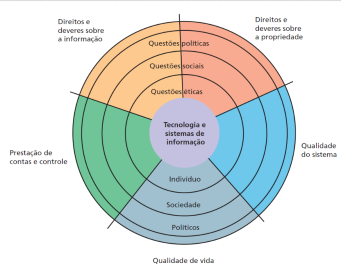
\includegraphics{fig2.png}}
\caption{Circulos Concêntricos de Laudon e Laudon}
\label{fig}
\end{figure}

Quando aplicado às plataformas de streaming audiovisual, podemos identificar algumas implicações éticas que abrangem um ou mais círculos.

\begin{itemize}
    \item Privacidade e vigilância: Como detalhado ao longo da seção \ref{sec: Recomendação: Coleta, Processamento e Armazenamento}, o sistema de recomendação baseia seu funcionamento a partir de dados obtidos dos usuários da plataforma de streaming. Essa coleta de dados constante pode implicar em questões relacionadas à privacidade do usuário. Essa questão, como já exemplificada no caso da Cambridge Analityca, já ultrapassou a amplitude individual e social, tendo em vista que já foram criadas medidas políticas para lidar com a situação \cite{b12}.
    \item Impacto Ambiental: O sistema de streaming audiovisual necessita para sua existência e funciomento de grandes equipamentos de hardware \ref{sec: Software, Hardware e Pessoas}, esse fato está associado com questões ambientais. Isso porque estima-se que um grande Centro de Dados de médio porte utiliza cerca de 300 mil galões de água por dia \cite{b13}. Esse impacto atinge diretamente a sociedade e necessita de um maior cuidado estatal para lidar com o problema.
    \item Manipulação e Desinformação: No livro \textit{O filtro invisível}, Eli Pariser \cite{b14} disserta sobre como as redes sociais, através de seus sistemas de recomendação, estão isolando os usuário em bolhas pessoais que limitam o alcance cultural, social e político destes em razão de suas próprias preferências. Esse fenômeno também pode ser estendido para as plataformas de streaming, que funcionam a partir da personalização da entrega de conteúdo. Tal questão está associada com o indivíduo mas também pode afetar a sociedade ao forçar (indiretamente) pessoas a consumir conteúdos de apenas um viés e, assim, gerar uma sociedade polarizada.
    
\end{itemize}


\section{Conclusão}
A investigação deste artigo confirma que as plataformas de streaming são, de fato, sistemas de informação conforme definidos por Laudon e Laudon \cite{b3}. Essas plataformas coletam dados sobre o comportamento dos usuários, processam essas informações para oferecer recomendações personalizadas, armazenam grandes volumes de conteúdo e informações de usuários, e disseminam dados de forma eficiente para otimizar a experiência do usuário.

Além disso, a capacidade dessas plataformas de adaptar e ajustar continuamente suas ofertas com base no feedback e nas preferências dos usuários demonstra a aplicação prática de um sistema de informação. Isso inclui a análise de grandes conjuntos de dados para identificar padrões e tendências, o que permite uma personalização cada vez mais precisa e uma descoberta contínua de novos conteúdos.

Portanto, ao integrar coleta, processamento, armazenamento e disseminação de informações, as plataformas de streaming exemplificam os princípios fundamentais de sistemas de informação. Elas não apenas suportam decisões e operações, mas também desenvolvem estratégias para melhorar a experiência do usuário e manter a relevância no mercado, sendo a principal ferramenta do atual cenário da indústria de entretenimento.

Por conseguinte, temos que essas plataformas moldaram a forma como consumimos produções culturais e audiovisuais. Tamanho impacto nos leva a imaginar as consequências que esses sistemas poderão gerar nas próximas gerações. Com base nesse viés, já é possível identificar alguns impactos causados, como as questões éticas discutidas anteriomente. Isto é, podemos concluir que o Streaming Audiovisual não só cumpre seu papel como Sistema de Informação mas também possui grande relevância na atual sociedade global, com questões a ser discutidas e um futuro promissor no ramo de entretenimento e comunicação.

\bibliographystyle{IEEEtran}
\bibliography{references}

\end{document}
